\chapter{基于网络流量和拓扑结构的关键横向移动流检测方法}{
{
\let\cleardoublepage\relax
}

攻击者进行横向移动时,通常会有关键的攻击行为可被发现,例如与集群 API 服务器的异常通信,旨在创建新的具有特权的 Pod。本章通过网络流量特征对关键流进行检测。

\section{容器化环境中的攻击链}

容器化集群中的资源通过 API 服务器进行增、删、改、查。因此,横向移动攻击的关键在于 API 服务器的通信。容器化环境中的攻击链\citep{armo2024}如图~\ref{fig:attack-1}~所示。

\begin{figure}[!htbp]
    \centering
    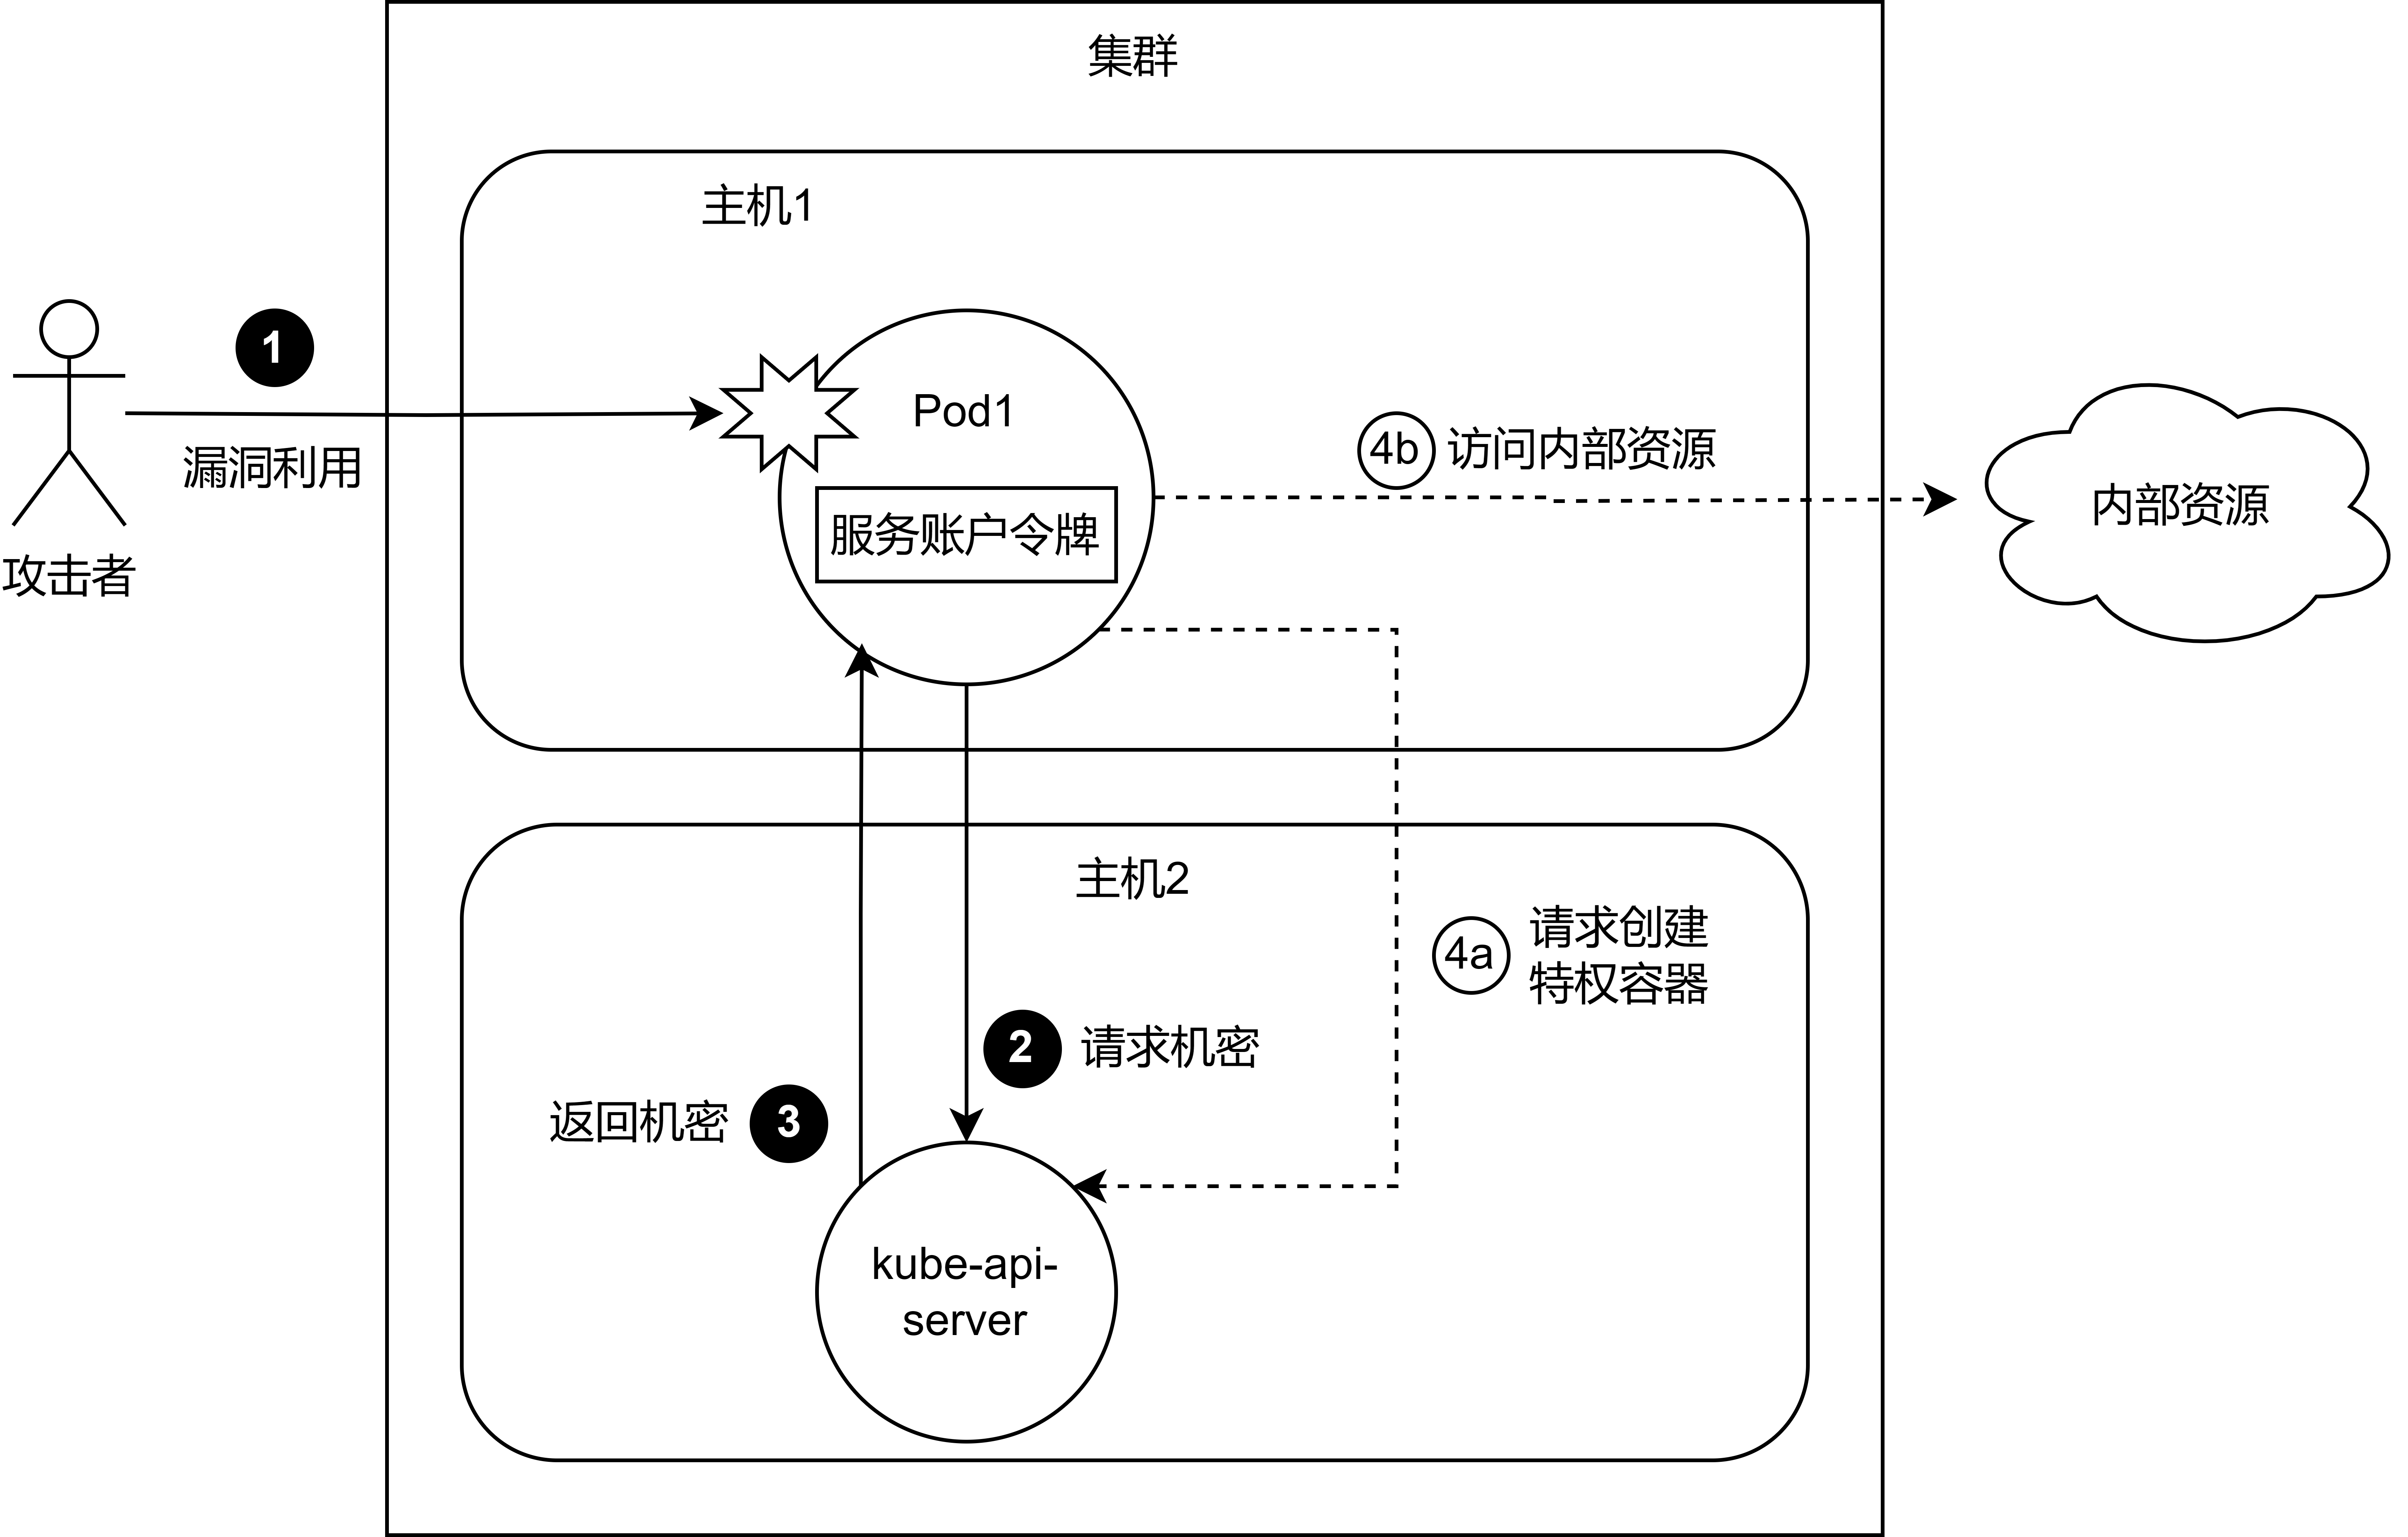
\includegraphics[width=0.95\textwidth]{attack-1}
    \bicaption{\enspace 容器化环境中的攻击链}{\enspace Attack Chain in Containerized Enviroments}
    \label{fig:attack-1}

\end{figure}

攻击链的各个阶段详细介绍如下:

\begin{enumerate}
    \item 攻击者进入目标集群。该阶段可通过远程代码执行漏洞实现,也可通过供应链攻击实现。攻击后,攻击者即可控制集群中的某个 Pod。
    \item 攻击者利用 Pod 中挂载的服务账户令牌,向集群 API 服务器请求身份认证。
    \item 集群 API 服务器对攻击者的身份认证通过。这是因为攻击者使用了 Pod 中的服务账户令牌,使 API 服务器不能识别攻击者的身份。
    \item 在这个阶段,攻击者尝试从当前的 Pod 移动到其他地方。图~\ref{fig:attack-1}~中给出了两个示例,其中第一个示例是创建一个新的特权 Pod,并将主机上的目录挂载到 Pod 中,从而实现从 Pod 到主机的横向移动;第二个示例是向 API 服务器请求机密信息,通过该机密信息,攻击者得以获得内部数据库等其他资源的访问权限。
\end{enumerate}

通过对攻击链的分析,本文发现,攻击者若要进行横向移动攻击,其最关键之处在于与 API 服务器之间的通信。攻击者需要与其通信,才能对集群的资源进行操作。因此,本文接下来将通过网络流量特征,对 API 服务器的异常通信进行检测,从而检测横向移动行为。

\section{基于网络流量特征的关键横向移动流检测方法}

本节基于网络流量特征检测关键横向移动流。检测流程如图~\ref{fig:detect-1}~所示。

\begin{figure}[!htbp]
    \centering
    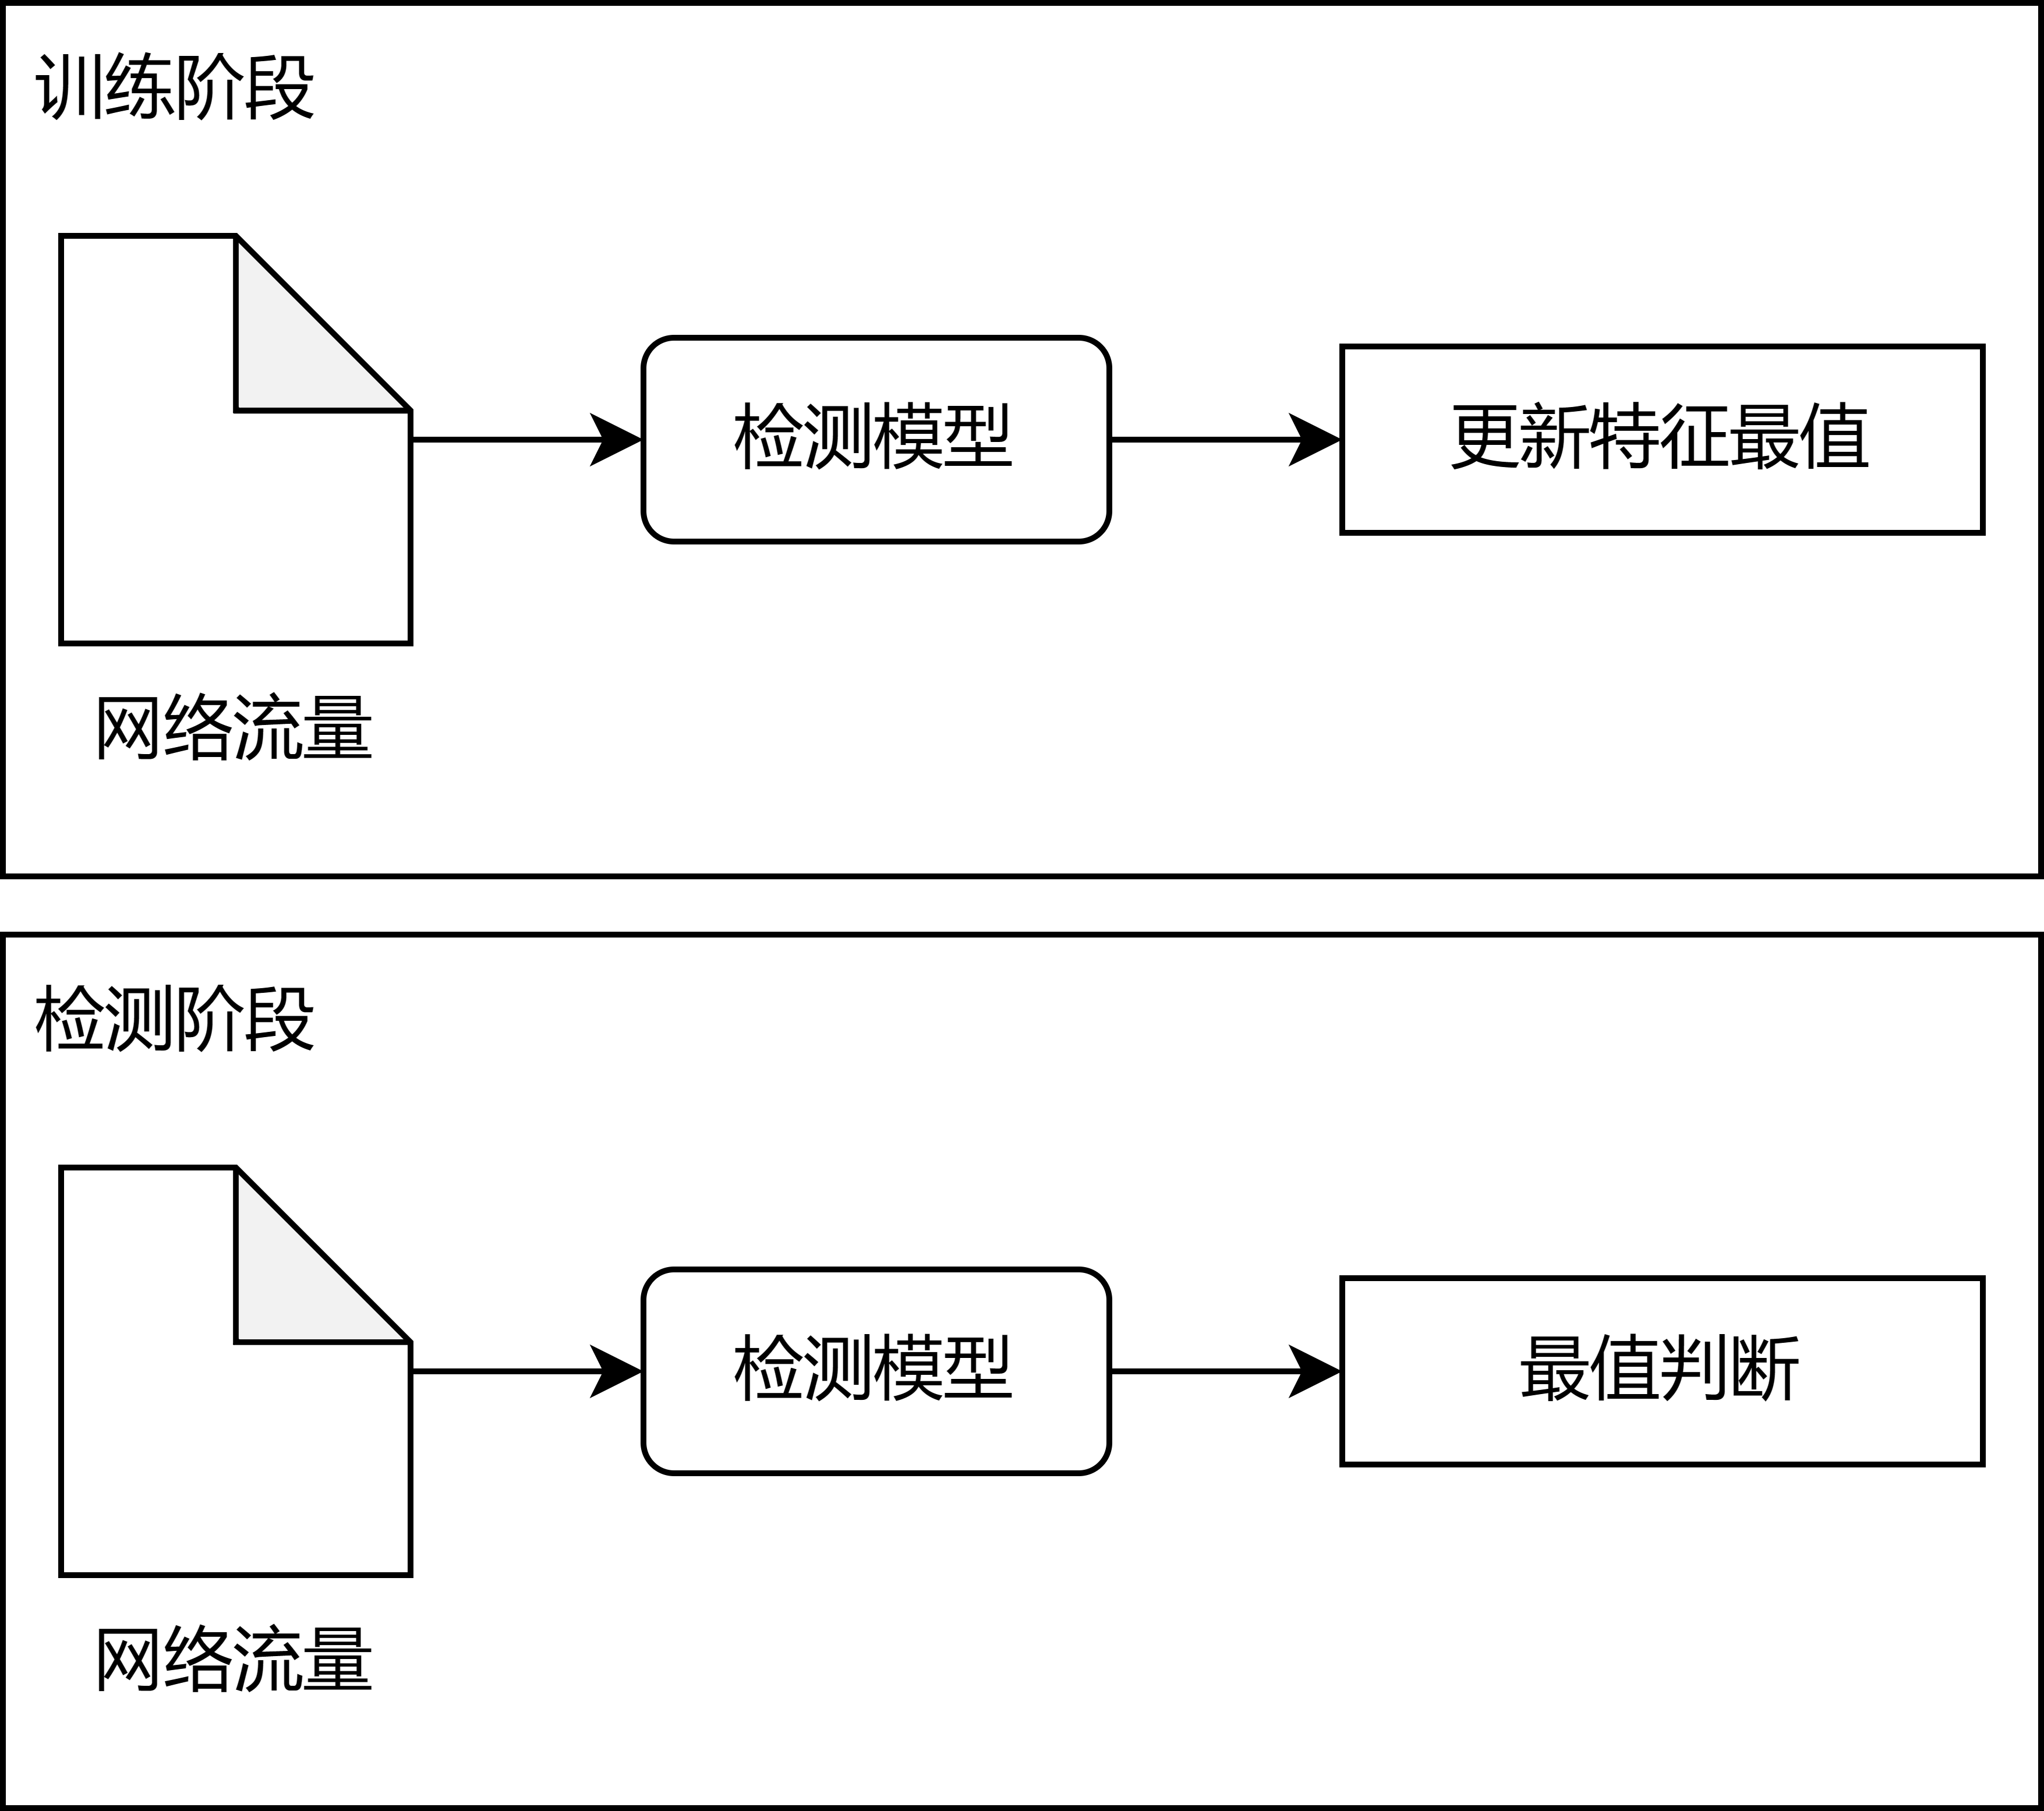
\includegraphics[width=0.50\textwidth]{detect-1}
    \bicaption{\enspace 基于网络流量特征的关键横向移动流检测流程}{\enspace Procedure of Detecting Key Flows of Lateral Movements by Flow Features}
    \label{fig:detect-1}

\end{figure}

该方法的基本思想是,当网络出现不同寻常的通信时,将报告异常。该方法通过特征最值来判断横向移动流。该方法分为两个阶段进行:

\begin{itemize}
    \item 训练阶段。在该阶段,读入网络流量的特征,更新网络流量特征的最值。
    \item 检测阶段。在该阶段,读入网络流量的特征,超出最值范围的判定为异常。
\end{itemize}

方法的伪代码如图~\ref{fig:detect-code}~所示。

\begin{figure}[!htbp]
    \centering
    \begin{subfigure}[b]{1.0\textwidth}
        \hrulefill
        \begin{algorithmic}[1]
            \Require NetflowList, FeatureList
            \Ensure MinMap, MaxMap
            \Function {TrainMap}{NetflowList, FeatureList}
                \State MinMap $\gets \emptyset$, MaxMap $\gets \emptyset$
                \For{Netflow \textbf{in} NetflowList}
                    \If{Netflow.SrcPort $\neq$ 6443 \textbf{or} Netflow.DstPort $\neq$ 6443}
                        \State \textbf{continue}
                    \EndIf
                    \For{Feature \textbf{in} FeatureList}
                        \State MinMap[Feature] $\gets $ Min (MinMap[Feature], Netflow[Feature])
                        \State MaxMap[Feature] $\gets $ Max (MinMap[Feature], Netflow[Feature])
                    \EndFor
                \EndFor
            \EndFunction
            \end{algorithmic}
        \hrulefill
        \caption{训练阶段}
    \end{subfigure}
    \\
    \begin{subfigure}[b]{1.0\textwidth}
        \hrulefill
            \begin{algorithmic}[1]
            \Require NetflowList, FeatureList, MinMap, MaxMap
            \Ensure Alerts
            \Function{TestFlow}{NetflowList, FeatureList, MinMap, MaxMap}
                \For{Netflow \textbf{in} NetflowList}
                    \If{Netflow.SrcPort $\neq$ 6443 \textbf{or} Netflow.DstPort $\neq$ 6443}
                        \State \textbf{continue}
                    \EndIf
                    \For{Feature \textbf{in} FeatureList}
                        \If{MinMap[Feature] $>$ Netflow[Feature] \textbf{or} MaxMap[Feature] $<$ Netflow[Feature]}
                            \State \textbf{alert} Netflow
                        \EndIf
                    \EndFor
                \EndFor
            \EndFunction
            \end{algorithmic}
        \hrulefill
        \caption{检测阶段}
    \end{subfigure}
    \bicaption{\enspace 基于网络流量特征的关键横向移动流检测伪代码}{\enspace Pseudocode of Detecting Key Flows of Lateral Movements}
    \label{fig:detect-code}
\end{figure}

\section{基于网络拓扑结构的关键横向移动流检测方法}

除了网络流量特征以外,攻击者的横向移动还会影响网络的拓扑结构。从容器化环境中的攻击链可以看出,攻击者可能通过新建特权 Pod 的形式实施 Pod 逃逸,以接管主机。在容器化集群中,每个 Pod 对应一个 IP 地址,因此新增 Pod 时,也会新增一个 IP 地址,从而更改了网络的拓扑结构。

此外,当攻击者攻破某一个 Pod 时,为了方便控制该 Pod,常用的方式是使用命令与控制服务器(Command and Control,C\&C)与该 Pod 进行通信。因此,该 Pod 将向其以前从未访问过的 IP 地址传输数据,从而更改了网络的拓扑结构。

因此,本文提出基于网络拓扑结构的关键横向移动流检测方法,检测流程如图~\ref{fig:detect-2}~所示。

\begin{figure}[!htbp]
    \centering
    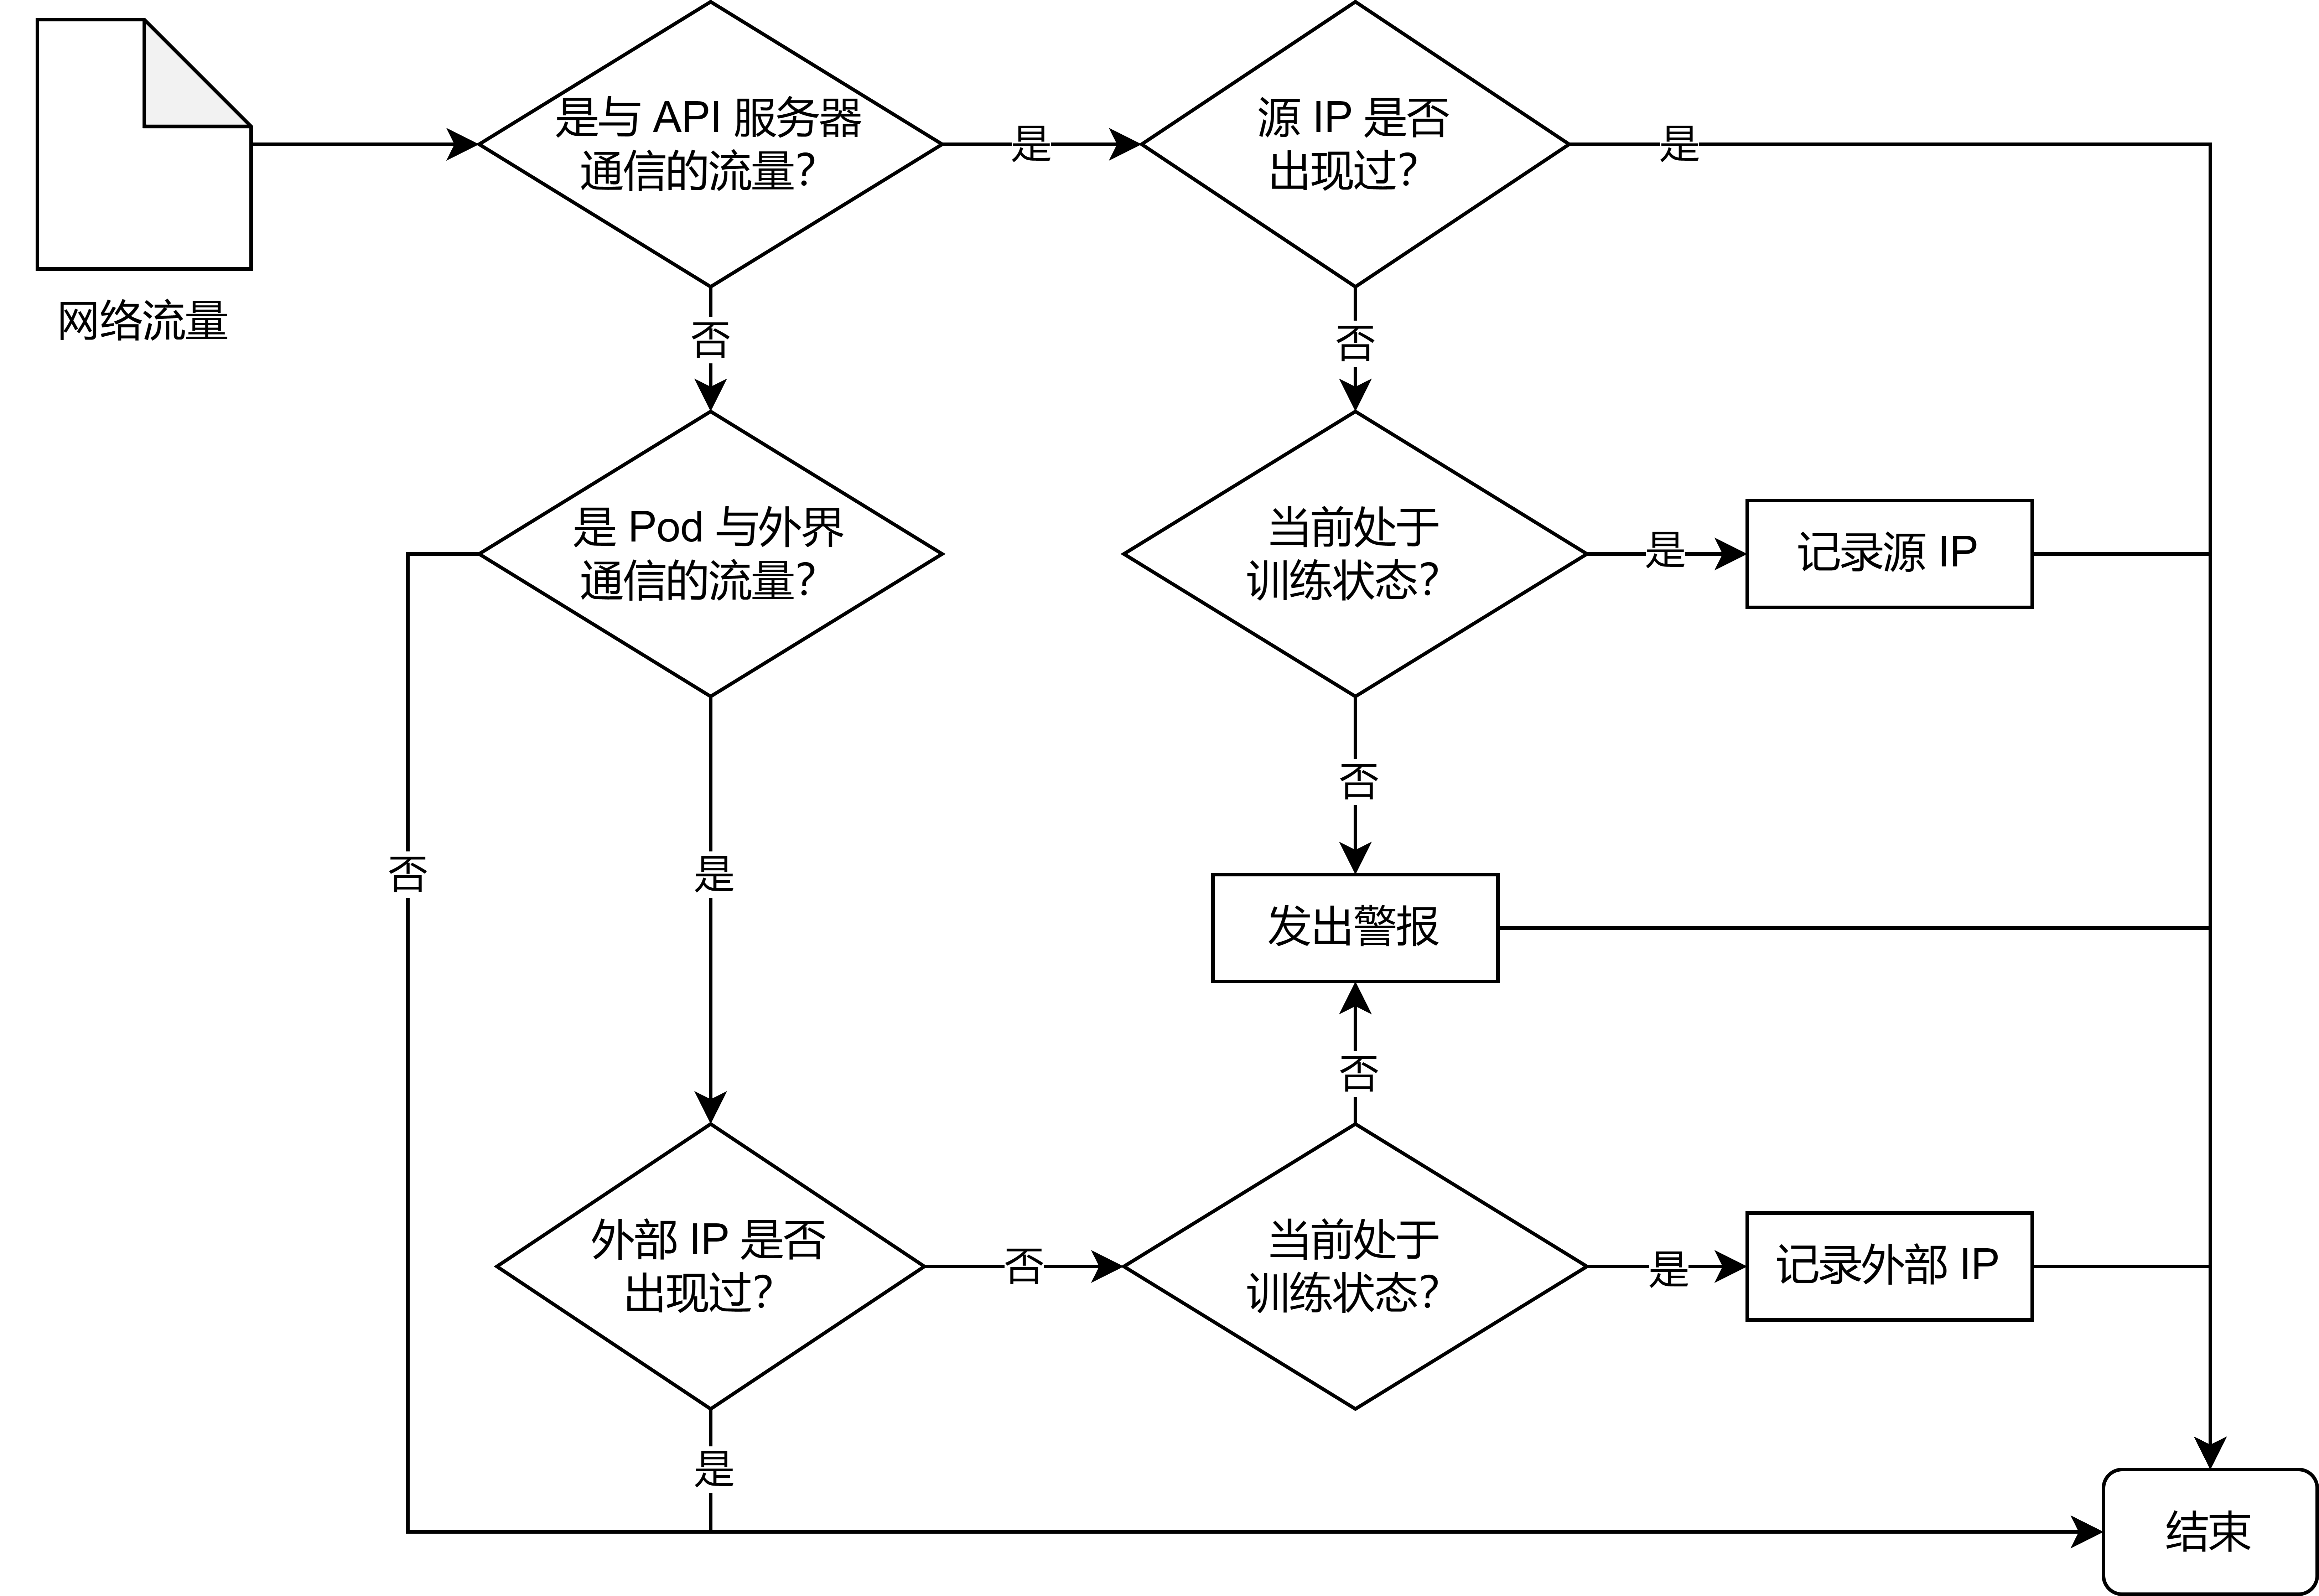
\includegraphics[width=1.0\textwidth]{detect-2}
    \bicaption{\enspace 基于网络拓扑结构的关键横向移动流检测流程}{\enspace Procedure of Detecting Key Flows of Lateral Movements by Topology}
    \label{fig:detect-2}

\end{figure}

其基本流程如下:

\begin{enumerate}
    \item 对于 API 服务器的通信,在训练阶段,记录通信的源 IP 地址;在检测阶段,检查通信的源 IP 地址是否在已记录的范围内,若未记录,则发出警报;
    \item 对于 Pod 与外部网络之间的通信,在训练阶段,记录通信的外部 IP 地址;在检测阶段,检查通信的外部 IP 地址是否在已记录的范围内,若未记录,则发出警报。
\end{enumerate}

实际应用时,根据具体部署的应用,可以对上述方法作适当调整,例如对于 Pod 与外部网络的通信,可以用域名来取代外部 IP 地址,使其更加准确;对于不需要与外部网络通信的 Pod,则可以简化策略,无需再训练阶段记录,而是在检测阶段直接检查该 Pod 是否与外部网络发生了通信,若发生了通信,则发出警报。

\section{数据集分析和验证}

本节使用 Kubernetes-dataset 数据集对关键横向移动流检测方法进行验证,其详细介绍见第~\ref{sec:dataset}~节。

\subsection{基于网络流量特征的方法验证}

Kubernetes-dataset 数据集中包含的网络流特征如表 ~\ref{tab:dataset-features}~ 所示。

\begin{table}[!htbp]
    \bicaption{\enspace Kubernetes-dataset 数据集包含的特征}{\enspace Features in Kubernetes-dataset}
    \label{tab:dataset-features}
    \centering
    \footnotesize% fontsize
    \setlength{\tabcolsep}{4pt}% column separation
    \renewcommand{\arraystretch}{1.2}%row space 
    \begin{tabular}{cp{10cm}c}
        \hline
        特征类别 & 特征 & 维度\\
        \hline
        流持续时间 & 流持续毫秒数、TCP流持续毫秒数 & 2\\
        数据包的数量 & 前向数据包数量、后向数据包数量、后向与前向数据包比例、含有至少1字节数据的数据包数量 & 4\\
        数据包的长度 & 前向数据包总长度、后向数据包总长度、前向数据包长度最大值、前向数据包长度最小值、前向数据包长度平均值、前向数据包长度标准差、后向数据包长度最大值、后向数据包长度最小值、后向数据包长度平均值、后向数据包长度标准差、数据包长度最小值、数据包长度最大值、数据包长度平均值、数据包长度标准差、数据包长度方差、平均数据包长度、前向数据段平均大小、后向数据段平均大小、前向数据段最小值 & 19\\
        流速 & 流速(包/秒)、流速(字节/秒)、前向流速(包/秒)、后向流速(包/秒)& 4\\
        数据包的间隔 & 数据包到达时间间隔(IAT)平均值、IAT标准差、IAT最大值、IAT最小值、前向IAT总和、前向IAT平均值、前向IAT标准差、前向IAT最大值、前向IAT最小值、后向IAT总和、后向IAT平均值、后向IAT标准差、后向IAT最大值、后向IAT最小值 & 14\\
        TCP Flag统计 & 前向PSH、后向PSH、前向URG、后向URG、前向RST、后向RST、FIN、SYN、RST、PSH、ACK、URG、CWR、ECE & 14\\
        数据包首部 & 前向首部长度、后向首部长度 & 2\\
        批量(bulk)传输 & 前向每bulk传输字节数、前向每bulk传输数据包数、前向bulk速率、后向每bulk传输字节数、后向每bulk传输数据包数、后向bulk速率	& 6\\
        MPTCP子流 & 前向子流数据包数、前向子流字节数、后向子流数据包数、后向子流字节数	& 4\\
        TCP窗口 & 前向窗口初始值、后向窗口初始值 & 2\\
        活跃与空闲 & 连续活跃时长平均值、连续活跃时长标准差、连续活跃时长最大值、连续活跃时长最小值、连续空闲时长平均值、连续空闲时长标准差、连续空闲时长最大值、连续空闲时长最小值 & 8\\
        \hline
    \end{tabular}
\end{table}

将数据集中的各个特征用散点图画出,可得到良性流量与横向移动流量各特征的分布情况。可以发现,部分特征在横向移动流量的值域大于良性流量的值域。符合这类分布的特征包括:前向每 bulk 传输字节数、前向每 bulk 传输数据包数、前向 bulk 速率。以前向每 bulk 传输字节数为例,横向移动流量和良性流量的散点图如图~\ref{fig:flow-bytes-bulk-avg}~所示。

\begin{figure}[!htbp]
    \centering
    \begin{subfigure}[b]{0.48\textwidth}
      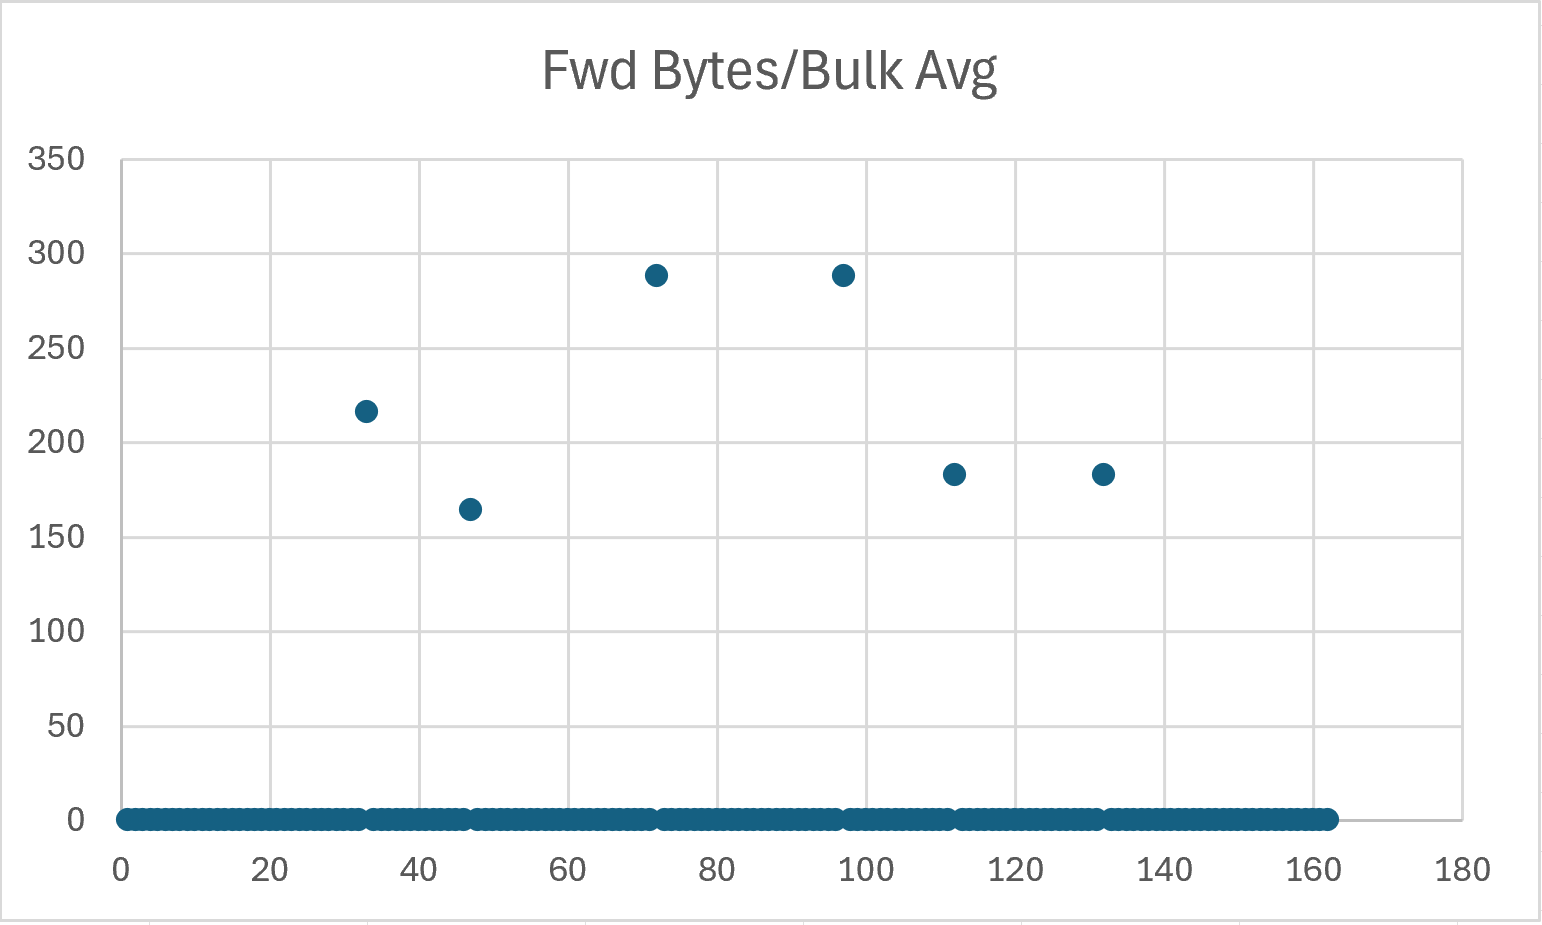
\includegraphics[width=\textwidth]{fwd-bytes-bulk-attack-1}
      \caption{横向移动流}
    \end{subfigure}%
    ~% add desired spacing
    \begin{subfigure}[b]{0.48\textwidth}
      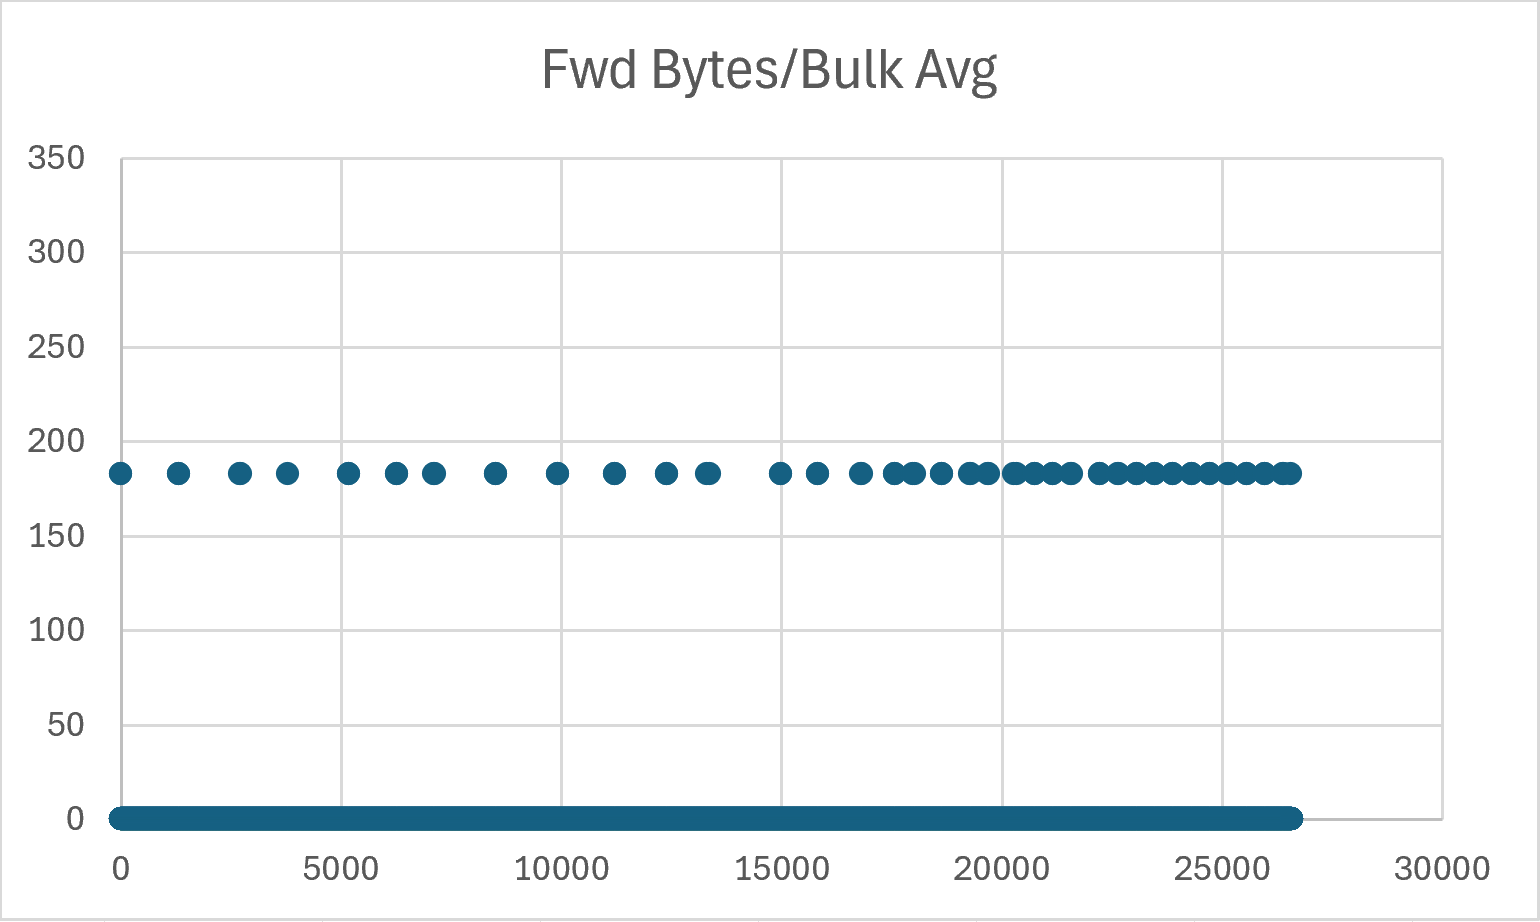
\includegraphics[width=\textwidth]{fwd-bytes-bulk-benign-1}
      \caption{良性流}
    \end{subfigure}
    \bicaption{\enspace 前向每 bulk 平均传输字节数散点图}{\enspace Scatterplot of Flow Bytes/bulk Average}
    \label{fig:flow-bytes-bulk-avg}
\end{figure}

在数据集中,若 TCP 流传输了大量数据,需分为多个数据包传输,这些数据包的集合就被称为 bulk。在进行流的聚合和特征提取时,CICFlowMeter 首先根据流中各数据包的发送时间间隔判断这些数据包能否被聚合为 bulk,然后统计数据包的数量,当数据包达到 4 个时就开始提取 bulk 的特征。因此,数据集中与 bulk 相关的特征通常为 $0$,仅在传输数据量较大时大于 $0$,表示此流发生了分包传输。

在图~\ref{fig:flow-bytes-bulk-avg}~所示的横向移动流中,共有$7$个流的前向数据发生了分包传输。这$7$个流的源IP地址、源端口、目标IP地址、目标端口如表~\ref{tab:dataset-malicious-bulks}~所示。

\begin{table}[!htbp]
    \bicaption{\enspace 横向移动流中发生分包传输的流}{\enspace Malicious Flows that Has Bulks}
    \label{tab:dataset-malicious-bulks}
    \centering
    \footnotesize% fontsize
    \setlength{\tabcolsep}{4pt}% column separation
    \renewcommand{\arraystretch}{1.2}%row space 
    \begin{tabular}{ccccccc}
        \hline
        编号 & 前向每 bulk 传输字节数 & 源 IP 地址 & 源端口 & 目标 IP 地址 & 目标端口 & 能否被检测出?\\
        \hline
        1 & 183 & 10.16.0.6 & 34788 & 144.122.71.18 & 6443 & 否\\
        2 & 183 & 10.16.0.2 & 56026 & 144.122.71.18 & 6443 & 否\\
        3 & 216 & 10.16.0.45 & 45956 & 144.122.71.18 & 6443 & 是\\
        4 & 164 & 10.16.0.45 & 47002 & 144.122.71.18 & 6443 & 是\\
        5 & 288 & 10.16.0.45 & 52904 & 144.122.71.18 & 6443 & 是\\
        6 & 288 & 10.16.0.45 & 52906 & 144.122.71.18 & 6443 & 是\\
        \hline
    \end{tabular}
\end{table}

与此同时,在良性流中,“前向每 bulk 传输字节数”大于 0 的流的情况如表~\ref{tab:dataset-benign-bulks}~所示。其中,具有相同或相似(除源端口以外其他特征相同)特征的流仅展示一次。

\begin{table}[!htbp]
    \bicaption{\enspace 良性流中发生分包传输的流}{\enspace Benign Flows that Has Bulks}
    \label{tab:dataset-benign-bulks}
    \centering
    \footnotesize% fontsize
    \setlength{\tabcolsep}{4pt}% column separation
    \renewcommand{\arraystretch}{1.2}%row space 
    \begin{tabular}{cccccc}
        \hline
        编号 & 前向每 bulk 传输字节数 & 源 IP 地址 & 源端口 & 目标 IP 地址 & 目标端口\\
        \hline
        7 & 183 & 10.16.0.6 & 34788 & 144.122.71.18 & 6443\\
        8 & 183 & 10.16.0.2 & 56026 & 144.122.71.18 & 6443\\
        \hline
    \end{tabular}
\end{table}

留意到良性流量中,向该端口传输数据的流的“前向每 bulk 传输字节数”通常为 183 字节,但横向移动流中出现了不同的值,说明 API 服务器接收到了与以往不相同的指令,而这正是横向移动攻击的关键。通过与 API 服务器通信,攻击者可以执行创建、更新、删除容器化集群中的 Pod 等资源,或者控制集群的行为,例如滚动更新、扩缩容等。因此,编号为 3、4、5、6 的 $4$ 个关键的横向移动流可通过此特征检测出来。

除了与 bulk 相关的特征以外,前向发送数据量、前向 PSH、前向首部长度等特征也可将这些流检测出来。

通过上述验证,本文证明了通过最值验证,可以检测出攻击者对 API 服务器的恶意操作,这是横向移动中的关键步骤。

(二)横向移动流量的值域与良性流量的值域大致相同。与IAT相关的特征,SYN、RST、FIN等与TCP协议握手、挥手过程相关的特征,前向初始窗口,前向数据段最小值属于此类。以IAT平均值为例,横向移动流和良性流的散点图如图~\ref{fig:flow-iat-mean}~所示。

\begin{figure}[!htbp]
    \centering
    \begin{subfigure}[b]{0.48\textwidth}
      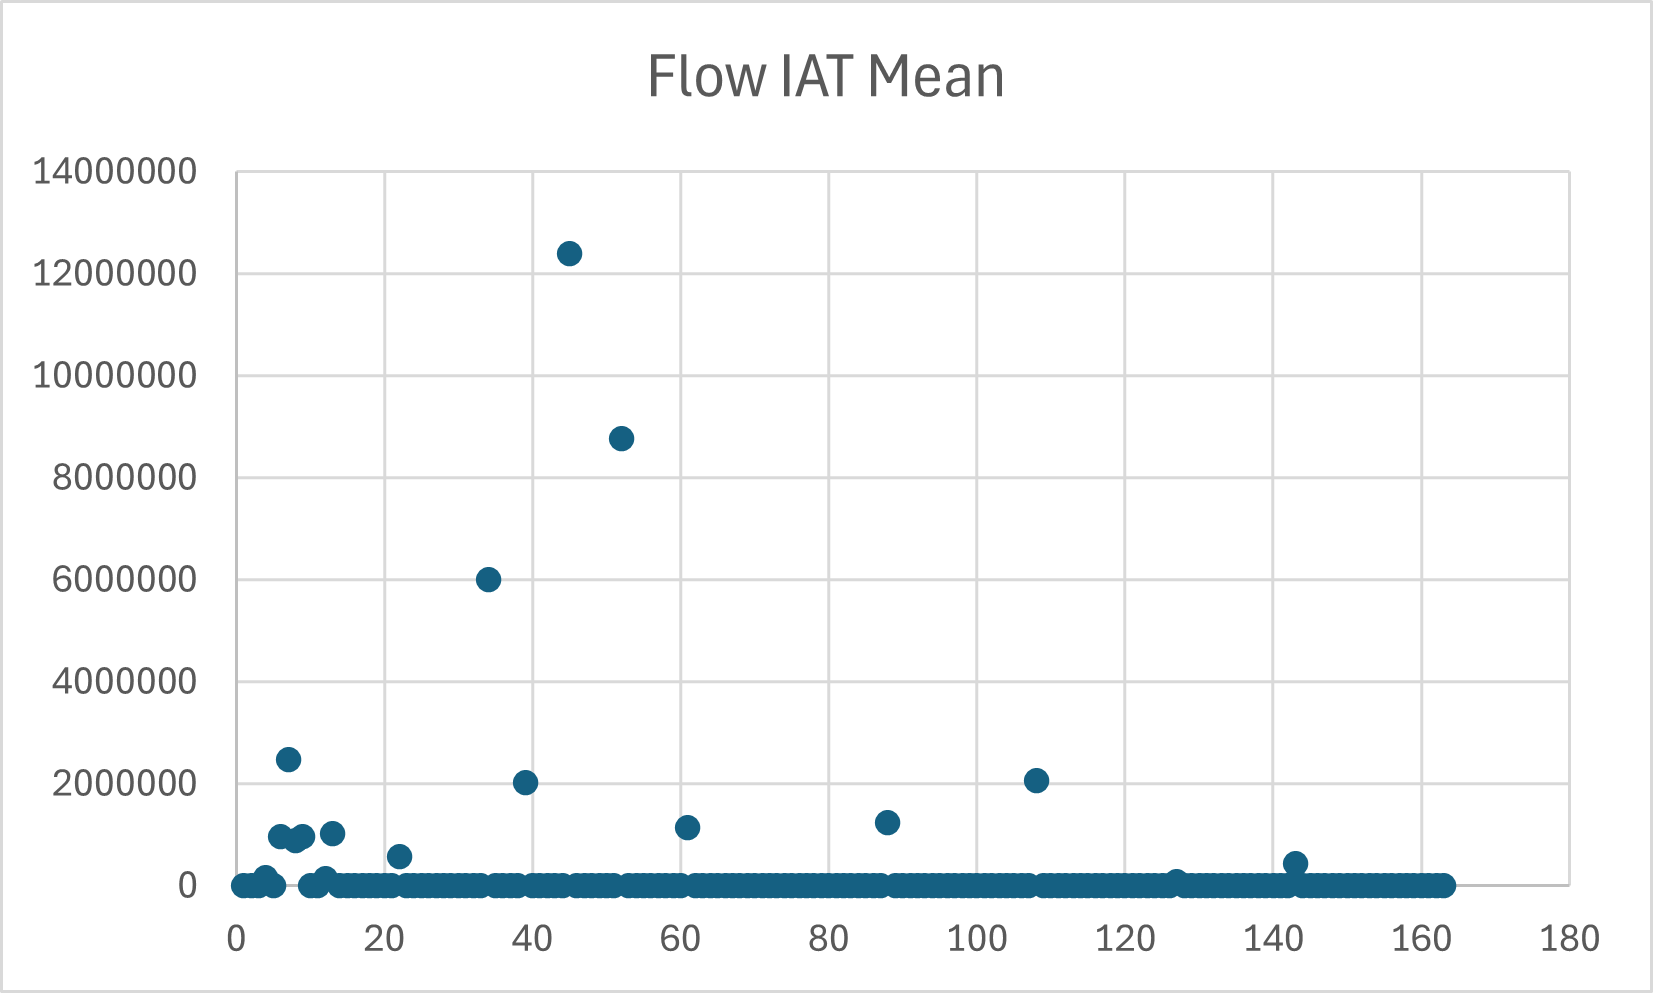
\includegraphics[width=\textwidth]{flow-iat-mean-attack}
      \caption{横向移动流}
    \end{subfigure}%
    ~% add desired spacing
    \begin{subfigure}[b]{0.48\textwidth}
      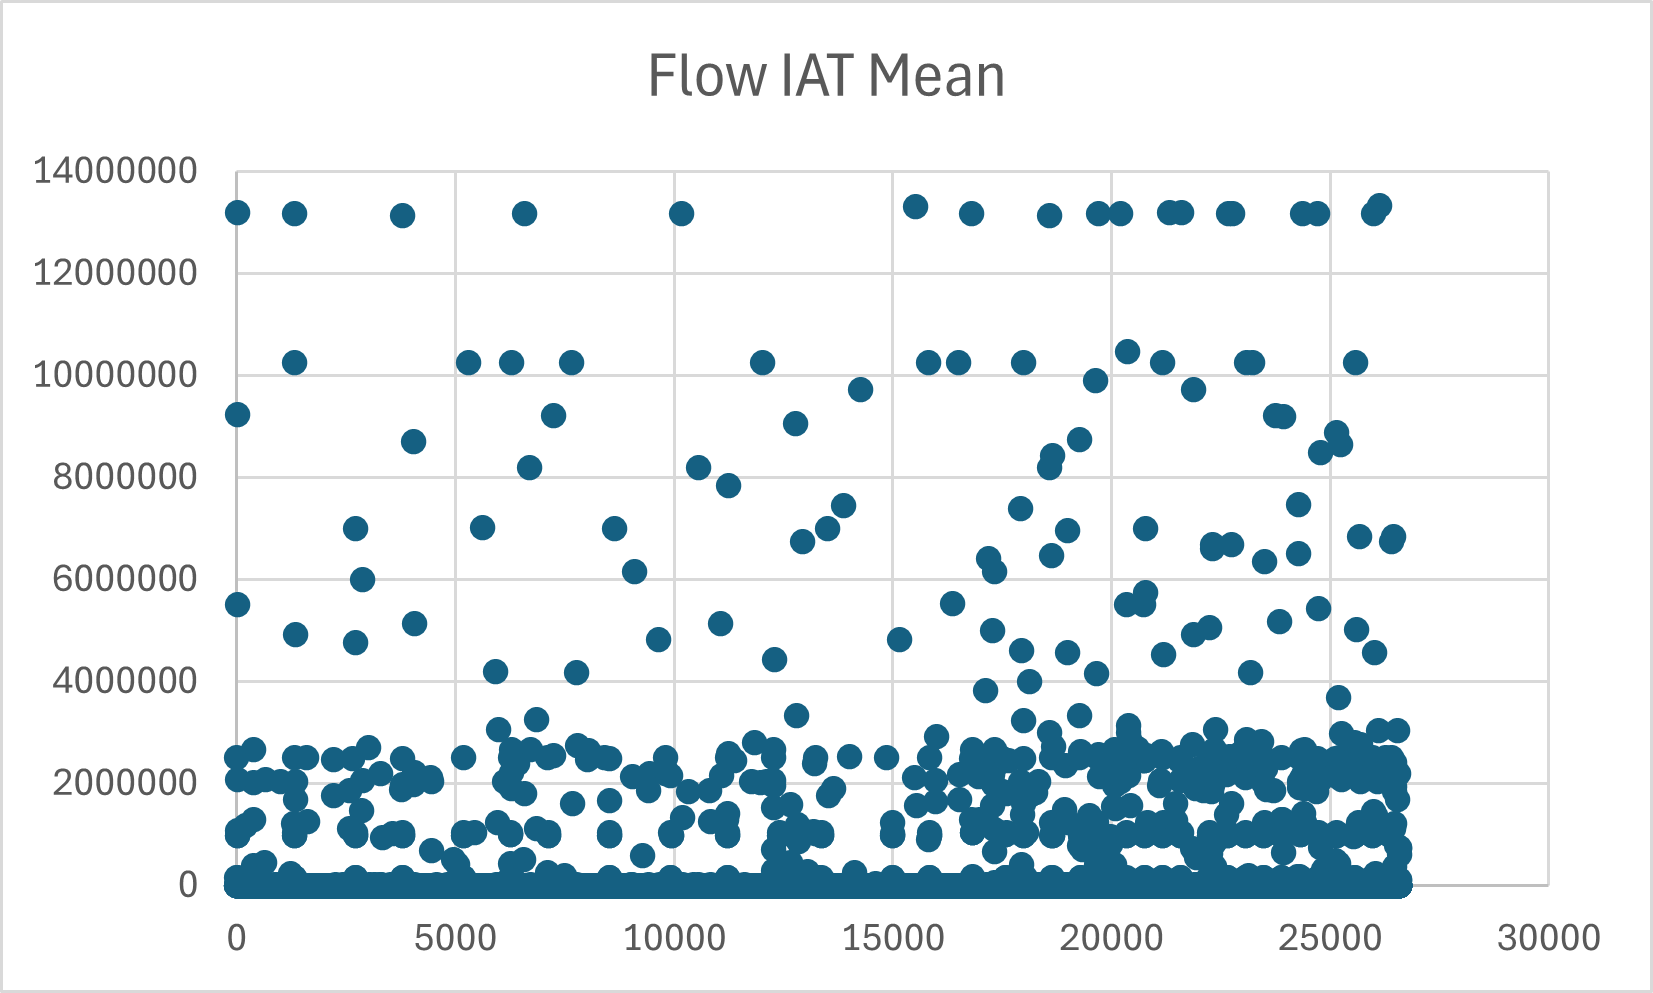
\includegraphics[width=\textwidth]{flow-iat-mean-benign}
      \caption{良性流}
    \end{subfigure}
    \bicaption{\enspace IAT 平均值散点图}{\enspace Scatterplot of IAT Mean}
    \label{fig:flow-iat-mean}
\end{figure}

此类特征难以区分横向移动流和良性流,因此难以直接用来识别横向移动。

(三)横向移动流量的值域小于良性流量的值域。与流持续时间、流速、包长相关且没有在(一)中讨论的特征属于此类。以流速为例,横向移动流量和良性流量的散点图如图~\ref{fig:flow-bytes}~所示。

\begin{figure}[!htbp]
    \centering
    \begin{subfigure}[b]{0.48\textwidth}
      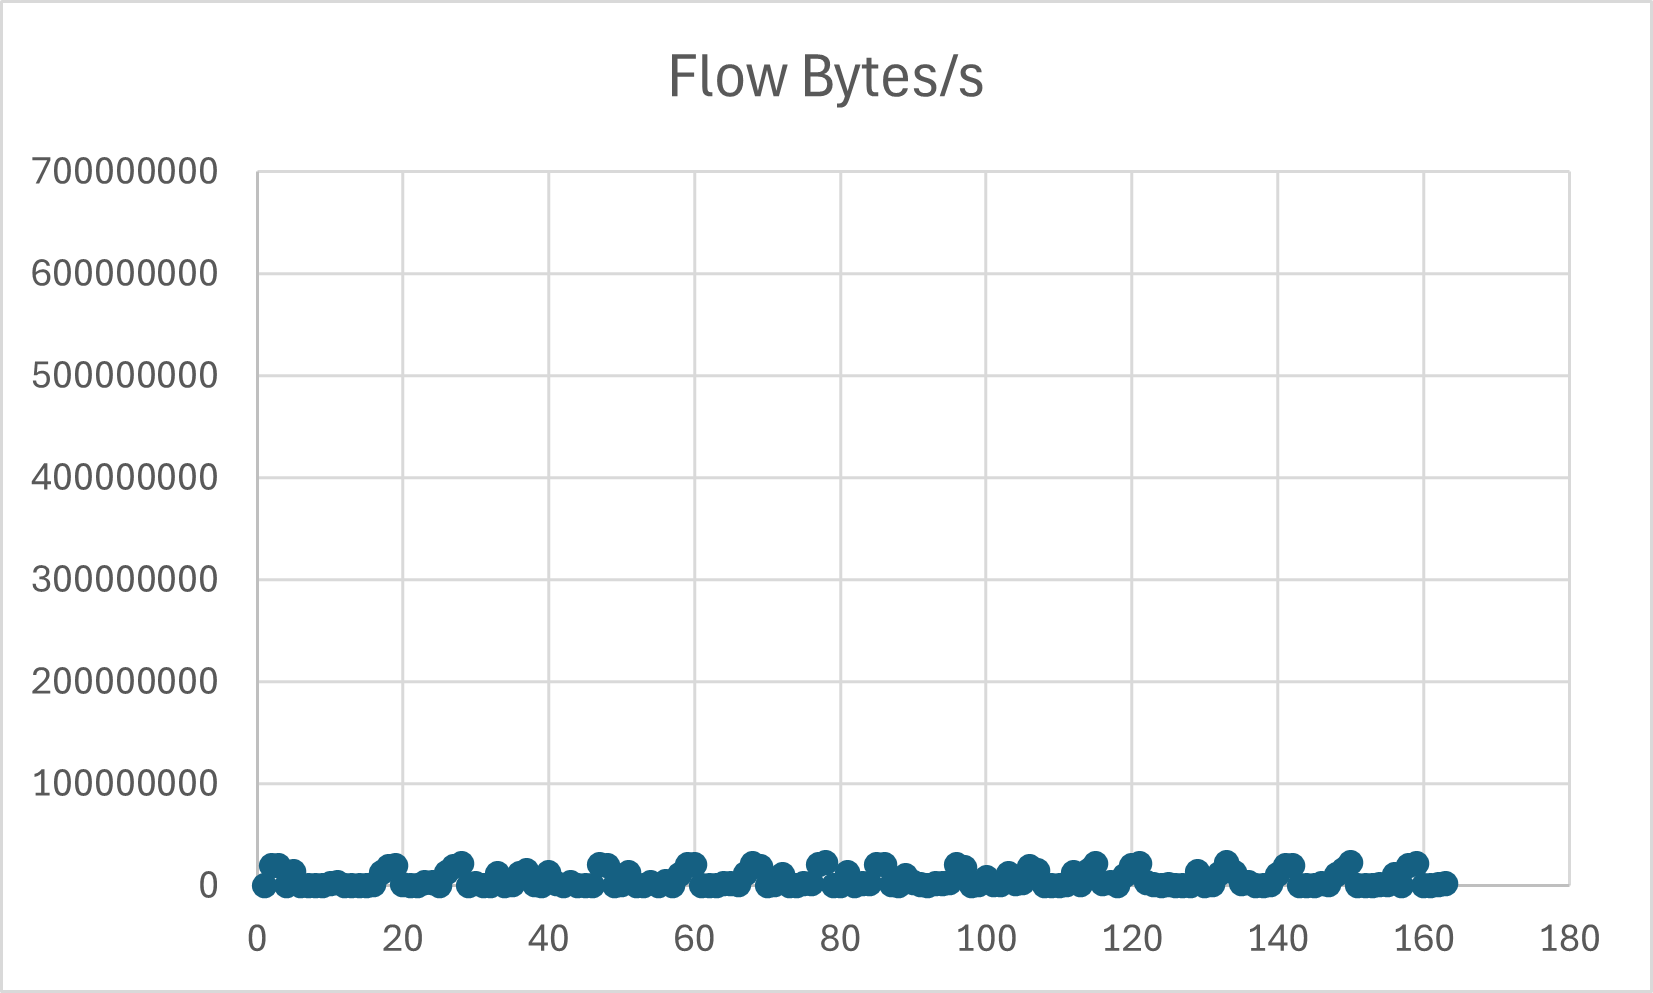
\includegraphics[width=\textwidth]{flow-bytes-attack}
      \caption{横向移动流}
    \end{subfigure}%
    ~% add desired spacing
    \begin{subfigure}[b]{0.48\textwidth}
      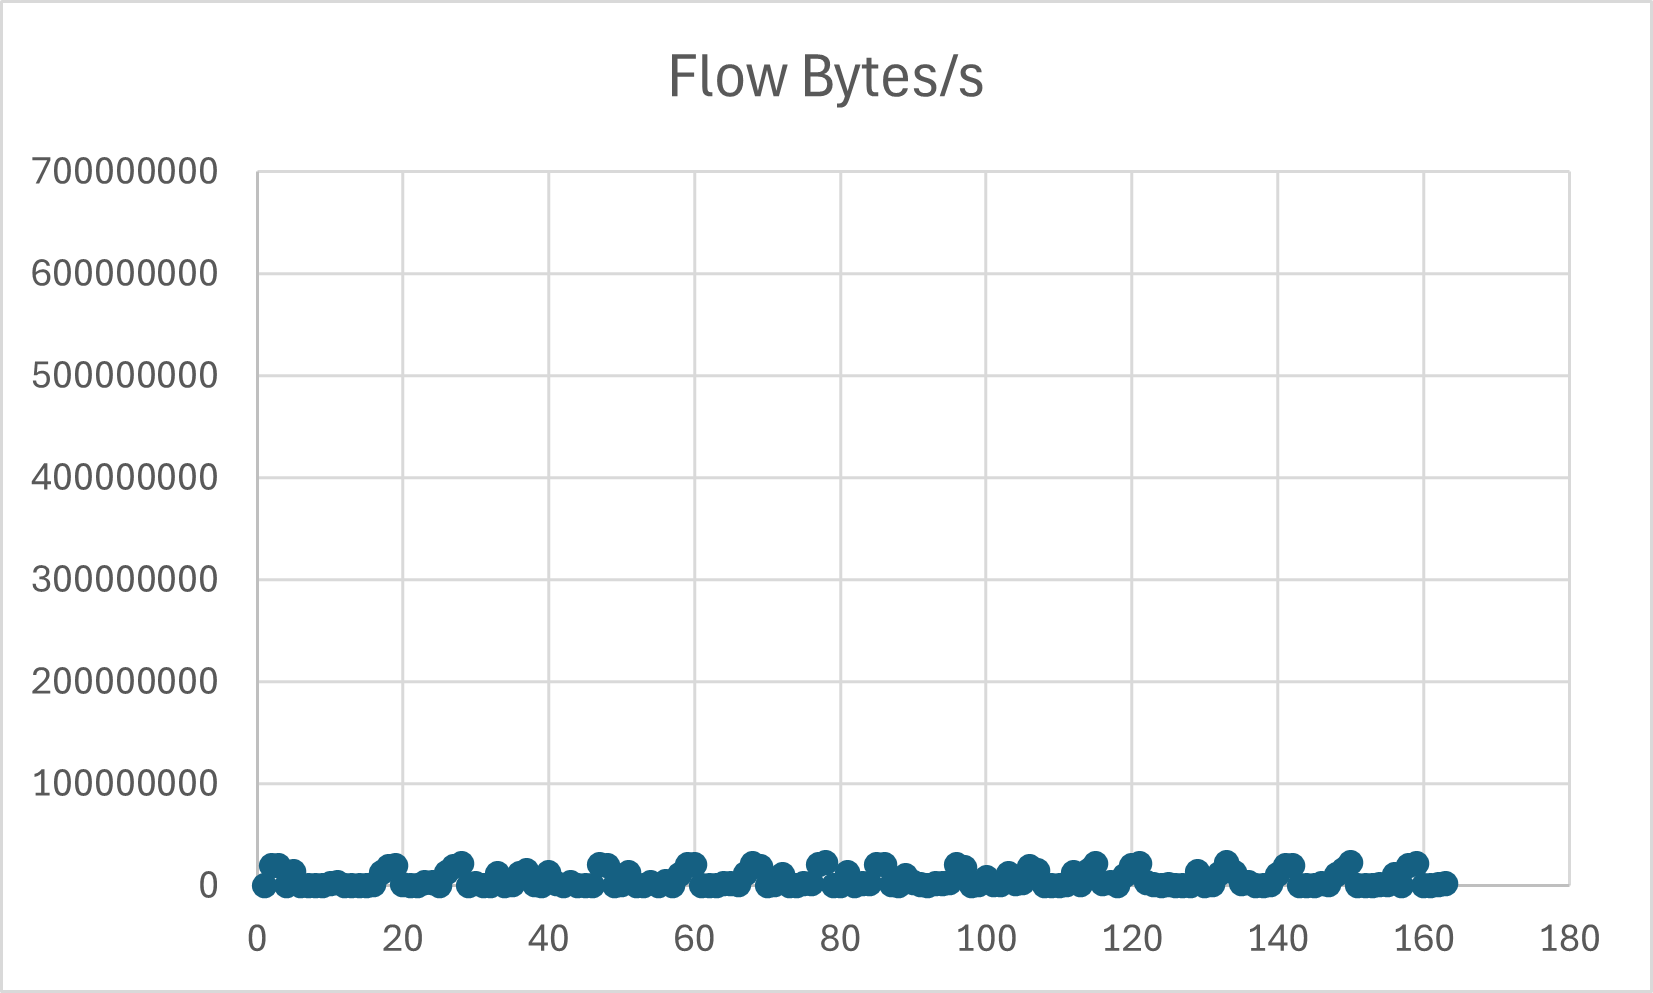
\includegraphics[width=\textwidth]{flow-bytes-attack}
      \caption{良性流}
    \end{subfigure}
    \bicaption{\enspace 流速散点图}{\enspace Scatterplot of Flow Rate}
    \label{fig:flow-bytes}
\end{figure}

此类特征同样难以区分横向移动流和良性流,因此难以直接用来识别横向移动。

因此,通过基于网络流量特征的最值检验,找出了横向移动中的 $5$ 个流,它们表示一个新建的 Pod 正在攻击者的控制下,向 API 服务器进行非法通信,进行恶意操作。然而,当这些流已经发生时才检测,往往为时已晚,最好在横向移动的更早阶段就能检测出来。因此,本节将基于机器学习进行网络流量特征筛选,为后续研究内容做好准备。

\subsection{基于网络拓扑结构的方法验证}

将网络流量的 IP 地址视为节点,节点之间的流量视为边,可以将网络流量以拓扑图的形式表现出来。数据集中良性流量的拓扑图如图~\ref{fig:benign-structure-ip}~所示。

\begin{figure}[!htbp]
    \centering
    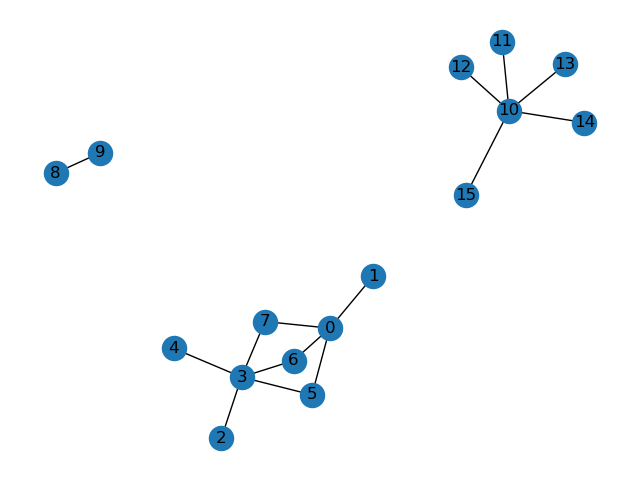
\includegraphics[width=0.75\textwidth]{benign-structure-ip}
    \bicaption{\enspace 良性流的网络拓扑结构}{\enspace Topological Diagram of Benign Flows}
    \label{fig:benign-structure-ip}

\end{figure}

包含良性流量和横向移动流量的拓扑图如图~\ref{fig:all-structure-ip}~所示。

\begin{figure}[!htbp]
    \centering
    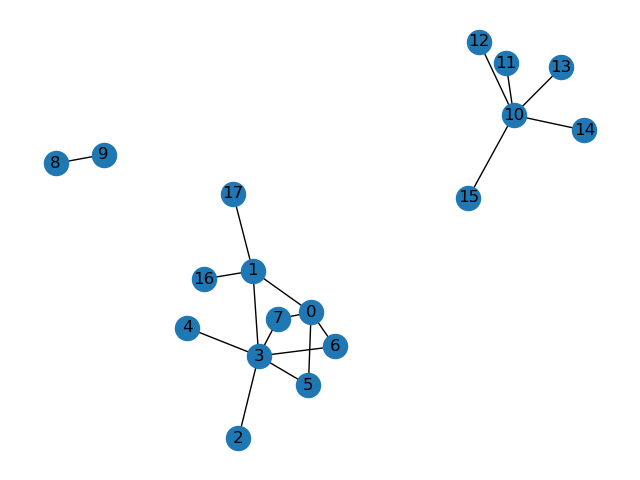
\includegraphics[width=0.75\textwidth]{all-structure-ip}
    \bicaption{\enspace 所有流的网络拓扑结构}{\enspace Topological Diagram of All Flows}
    \label{fig:all-structure-ip}

\end{figure}

图~\ref{fig:benign-structure-ip}~和图~\ref{fig:all-structure-ip}~中各节点所对应的 IP 地址如表~\ref{tab:cross-reference}~所示。

\begin{table}[!htbp]
    \bicaption{\enspace 节点与 IP 地址对照表}{\enspace Cross-reference Between Nodes and IP Addresses}
    \label{tab:cross-reference}
    \centering
    \footnotesize% fontsize
    \setlength{\tabcolsep}{4pt}% column separation
    \renewcommand{\arraystretch}{1.2}%row space 
    \begin{tabular}{cccccc}
        \hline
        编号 & IP 地址 & 备注\\
        \hline
        0 & 100.64.0.2 & 主机节点\\
        1 & 10.16.0.45 & 带有 Node-RED 软件的 Pod 节点\\
        2 & 10.16.0.2 & Pod 节点\\
        3 & 144.122.71.18 & API 服务器节点\\
        4 & 10.16.0.6 & Pod 节点\\
        5 & 10.16.0.5 & Pod 节点\\
        6 & 10.16.0.4 & Pod 节点\\
        7 & 10.16.0.7 & Pod 节点\\
        8 & 10.16.0.9 & Pod 节点\\
        9 & 18.165.61.116 & 外部节点\\
        10 & 10.16.0.18 & Pod 节点\\
        11 & 34.120.177.193 & 外部节点\\
        12 & 185.199.111.133 & 外部节点\\
        13 & 185.199.108.133 & 外部节点\\
        14 & 185.199.110.133 & 外部节点\\
        15 & 185.199.109.133 & 外部节点\\
        16 & 144.122.71.36 & 外部节点\\
        17 & 95.179.254.105 & 外部节点\\
        \hline
    \end{tabular}
\end{table}

通过图~\ref{fig:benign-structure-ip}~和图~\ref{fig:all-structure-ip}~的对比,可以看出,在正常情况下,节点 1 既不与外部节点通信,也不与 API 服务器通信。然而,当攻击者发起攻击后,节点 1 开始同时与外部节点和 API 服务器通信,这表明攻击者侵入 Node-RED 所在的 Pod 之后,操纵其向 API 服务器执行非法操作。因此,节点 1 与 API 服务器的通信和节点 1 与外部网络之间的通信均应发出警报,这对应 8 个流,具体如表~\ref{tab:dataset-topology-detect}~所示。

\begin{table}[!htbp]
    \bicaption{\enspace 基于网络拓扑结构的方法检出的横向移动流}{\enspace Malicious Flows Detected by Method Based on Topology}
    \label{tab:dataset-topology-detect}
    \centering
    \footnotesize% fontsize
    \setlength{\tabcolsep}{4pt}% column separation
    \renewcommand{\arraystretch}{1.2}%row space 
    \begin{tabular}{ccccccc}
        \hline
        源 IP 地址 & 源端口 & 目标 IP 地址 & 目标端口 & 能否被检测出?\\
        \hline
        144.122.71.36 & 9001 & 10.16.0.45 & 48754 & 是\\
        10.16.0.45 & 45956 & 144.122.71.18 & 6443 & 是\\
        10.16.0.45 & 46988 & 144.122.71.18 & 6443 & 是\\
        10.16.0.45 & 47002 & 144.122.71.18 & 6443 & 是\\
        10.16.0.45 & 52904 & 144.122.71.18 & 6443 & 是\\
        10.16.0.45 & 52906 & 144.122.71.18 & 6443 & 是\\
        10.16.0.45 & 54902 & 144.122.71.36 & 9001 & 是\\
        10.16.0.45 & 59624 & 95.179.254.105 & 443 & 是\\
        \hline
    \end{tabular}
\end{table}

\section{本章小结}

本章通过最值检测和拓扑分析的方式,将横向移动最关键阶段检测出来。在这个阶段,攻击者操控他所入侵的 Pod,与 API 服务器进行非法通信,以便进一步进行机密窃取、操控集群等行为。

然而,仅仅检测最关键阶段是不够的。如果在这个阶段才进行检测,往往为时已晚,因此我们需要在横向移动更早期的阶段就进行检测。这将在下一章中讨论。

}